\documentclass[apuntes]{subfiles}

\begin{document}

\section{Estructuras algebráicas, campos y espacios vectoriales} \label{Sec: Estructuras algebráicas, campos y espacios vectoriales}

El álgebra lineal se puede definir como el estudio de los espacios vectoriales. En esta sección definiremos qué son, así como algunas nociones básicas que guiarán nuestro estudio de este tipo de estructuras algebráicas durante el curso. Antes, discutiremos brevemente qué constituye una estructura algebráica y repasaremos la definición de la estructura de campo \textemdash necesaria para definir la de espacio vectorial.

\subsection*{Estructuras algebráicas} \label{Subsec: Estructuras algebráicas}

¿Qué es el álgebra, y qué es lo que estudia? A menudo en los primeros cursos de álgebra esta cuestión no queda clara. El hecho de que esta área de las matemáticas tenga una historia de evolución que comenzó hace miles de años y continúa hasta hoy en día complica aún más la situación. A pesar de no ser la visión más general que existe, en este curso tomaremos por respuesta que el álgebra es el estudio de estructuras algebráicas.

\subsubsection*{Definición de estructura algebráica y propiedades de sus operaciones} \label{Sssec: Definición de estructura algebráica y propiedades de sus operaciones}

\begin{tcolorbox}
    \underline{Def.} Una \emph{estructura algebráica} es un conjunto no vacío $A$ con (al menos) una operación en $A$ y una colección (posiblemente vacía) de relaciones en $A$. Denotamos a una estructura algebráica formada por un conjunto $A$, operaciones $\star,\ast$ y una relación $\sim$, como $(A,\star,\ast,\sim)$. Decimos que:

    \begin{itemize}
        \item $\star$ es \emph{binaria} si toma \textbf{pares ordenados} de elementos de $A$ y devuelve elementos de $A$, i.e., si su dominio es $A\times A$ y su contradominio es $A$, lo que denotamos como $\star:A\times A\to A$;

        \item $\star$ es \emph{asociativa} si, para cualesquiera $a,b,c\in A$, se tiene que $$(a\star b)\star c = a\star(b\star c);$$

        \item $\star$ es \emph{conmutativa} si, para cualesquiera $a,b\in A$, se tiene que $$a\star b = b\star a;$$

        \item $\star$ tiene un elemento \emph{identidad} (o \emph{neutro}) si existe $e\in A$ tal que, para todo $a\in A$, $$e\star a = a = a\star e;$$

        \item $b\in A$ es el elemento \emph{inverso} de $a\in A$ (\emph{bajo} $\star$) si $\star$ tiene un elemento identidad $e\in A$ y $$a\star b = e = b\star a;$$

        \item $B\subseteq A$ es \emph{cerrado bajo la operación} $\star$ si, para cualesquiera $x,y\in B$, $$x\star y\in B;$$

        \item $\star$ se \emph{distribuye con respecto a} $\ast$ si ambas operaciones son operaciones binarias y, para cualesquiera $a,b,c\in A$, $$a\star(b\ast c) = (a\star b)\ast(a\star c) \quad \& \quad (b\ast c)\star a = (b\star a)\ast(c\star a).$$
    \end{itemize}
\end{tcolorbox}
    
Observemos que, por definición, la relación de ``ser inverso bajo una operación'' es simétrica. Es decir, $a$ es inverso de $b$ bajo la operación $\star$ si, y sólo si, $b$ es inverso de $a$ bajo $\star$. Más aún, por definición, el elemento identidad de una operación, si existe, siempre es su propio inverso bajo esa operación. Frecuentemente diremos simplemente \emph{identidad} o \emph{neutro} para referirnos al elemento identidad de una operación. Así mismo, utilizaremos sólo la palabra \emph{estructura} para referirnos a una estructura algebráica. 

\subsubsection*{Ejemplos de estructuras algebráicas} \label{Sssec: Ejemplos de estructuras algebráicas}

Para cualquier conjunto arbitrario $A$, su conjunto potencia $\mathscr{P}(A)$ junto con las operaciones de unión e intersección de conjuntos ($\cup$ y $\cap$, respectivamente) y la relación ``contención'' ($\subseteq$) forma una estructura algebráica, que podemos escribir explícitamente como $(\mathscr{P}(A),\cup,\cap,\subseteq$). Observemos que ambas operaciones son binarias, asociativas y conmutativas, como seguramente viste en tu curso de Álgebra.

\begin{ejer}\label{ejercicio-1}
    Consideremos la estructura algebráica $(\mathscr{P}(A),\cup,\cap,\subseteq)$, donde $A$ es un conjunto arbitrario. ¿Quienes son los elementos neutros de $\cup$ y $\cap$? Demuéstralo.
\end{ejer}

El conjunto de los números naturales ($\mathbb{N}$) junto con la operación de suma ($+$) y la relación ``menor o igual que'' ($\le$) forma una estructura algebráica $(\mathbb{N},+,\le)$. Observemos que, en este caso, $+$ es una operación binaria, asociativa y conmutativa. Si incluimos al número $0$ en el conjunto $\mathbb{N}$, entonces $0$ es el elemento identidad de la suma, y es el único elemento de $\mathbb{N}$ que tiene inverso (¿Por qué?).

\begin{ejer}\label{ejercicio-2}
    Consideremos la estructura algebráica $(\mathbb{N},+,\le)$. Demuestra que ningún subconjunto finito $F$ de $\mathbb{N}$ es cerrado bajo la suma.
\end{ejer}

El conjunto de los números enteros junto con las operaciones de suma y multiplicación forma una estructura algebráica $(\mathbb{Z},+,\cdot)$. Similarmente, los conjuntos de los números racionales y los reales con las mismas operaciones \textemdash entre números racionales y reales, respectivamente\textemdash \ forman las estructuras $(\mathbb{Q},+,\cdot)$ y $(\mathbb{R},+,\cdot)$. Claramente, estas tres estructuras son distintas, pues los conjuntos que los forman son distintos. Sin embargo, $(\mathbb{Q},+,\cdot)$ y $(\mathbb{R},+,\cdot)$ forman el mismo \emph{tipo} de estructura algebráica puesto que, como veremos más adelante, sus operaciones cumplen las mismas propiedades. Estudiaremos este tipo de estructura, conocida como \emph{campo}, en la sección \ref{Ssec: Campos} como un primer paso hacia la definición de otro tipo de estructura conocida como \emph{espacio vectorial}, que definiremos en \ref{Ssec: Espacios vectoriales}. Además, veremos que no se necesitan relaciones para definir a estos tipos de estructuras. Por lo tanto, de ahora en adelante asumiremos que nuestras estructuras algebráicas no tienen relaciones. \\

Antes de definir estos tipos de estructuras algebráicas, veremos algunas nociones generales de estructuras que usaremos tanto en campos como en espacios vectoriales.

\subsubsection*{Unicidad de identidades e inversos} \label{Sssec: Unicidad de identidades e inversos}
    
\begin{prop}
    Sean $(A,\star)$ una estructura algebráica y $e\in A$ un elemento identidad de la operación $\star$. Entonces

    \begin{enumerate}[label=(\alph*)]
        \item $e$ es único;

        \item si la operación $\star$ es asociativa y $a\in A$ tiene un inverso $b$ bajo $\star$, entonces $b$ es único.
    \end{enumerate}
\end{prop}
    
\begin{proof}\leavevmode
    
    \begin{enumerate}[label=(\alph*)]

        \item Supongamos que $e'\in A$ es un elemento identidad de $\star$. Entonces $e=e\star e'=e'$. Por lo tanto, el elemento identidad $e$ de $\star$ es único.

        \item Supongamos que $\star$ es asociativa, $a\in A$ y que existe $b\in A$ tal que $b$ es inverso de $a$ bajo $\star$. Adicionalmente, supongamos que $b'\in A$ es un inverso de $a$ bajo $\star$. Entonces
            \begin{align*}
                b &= b\star e \tag{$e$ es neutro} \\
                  &= b\star (a\star b') \tag{$b'$ es inverso de $a$} \\
                  &= (b\star a)\star b' \tag{$\star$ es asociativa} \\
                  &= e\star b' \tag{$b$ es inverso de $a$} \\
                  &= b'.
            \end{align*}
            Por lo tanto, los elementos inversos bajo $\star$, si existen, son únicos.
    \end{enumerate}
\end{proof}

\subsubsection*{Funciones que preservan estructura} \label{Sssec: Funciones que preservan estructura}

Las estructuras no sólo se pueden estudiar a través de las interacciones de sus operaciones con \emph{elementos}, sino también a través de sus interacciones con \emph{funciones}. Sin embargo, trabajar con funciones \emph{arbitarias} para estudiar estructuras puede ser de poca utilidad. Un tipo de funciones muy útiles para estudiar la relación entre dos estructuras algebráicas son aquellas que \textbf{presevan su estructura}.

\begin{tcolorbox}
    
    \underline{Def.} Sean $(A,\star)$ y $(B,\diamondsuit)$ estructuras algebráicas. Decimos que una función $f:A\to B$ es \emph{compatible con las operaciones} $\star$ \emph{y} $\diamondsuit$ si, para todo $x,y\in A$, se cumple que
    \[
        f(x\star y) = f(x)\diamondsuit f(y).
    \]
    \noindent En este caso, también decimos que la función $f$ \emph{preserva la estructura} de $(A,\star)$ y $(B,\diamondsuit)$. \\

    En caso de que tengamos estructuras algebráicas con dos operaciones $(A,\star,\ast)$ y $(B,\diamondsuit,\spadesuit)$, diremos que una función $f:A\to B$ \emph{preserva su estructura} si es compatible con los pares de operaciones $(\star,\diamondsuit)$ y $(\ast,\spadesuit)$, i.e., si, para todo $x,y\in A$, se cumple que
    \begin{align*}
        f(x\star y) &= f(x)\diamondsuit f(y) \\
                    & \ \& \\
        f(x\ast y) &= f(x)\spadesuit f(y).
    \end{align*}
\end{tcolorbox}

\subsection*{Campos} \label{Ssec: Campos}

Un campo es un tipo de estructura algebráica que formaliza varias de las nociones intuitivas que adquirimos durante nuestra educación básica sobre la aritmética en los números reales; esto es, que la suma y la multiplicación son operaciones binarias, asociativas y conmutativas, que la multiplicación se distribuye con respecto a la suma, y que el $0$ y el $1$ son números ``especiales'' en cierto sentido, el cual precisaremos más adelante. \\

Quizá viste este tipo de estructura explícitamente en tu curso de Álgebra y/o implícitamente en tu curso de Cálculo I (a través de los \textit{axiomas de campo} \textemdash o \emph{de cuerpo}\footnote{En francés, este tipo de estructura es llamado \emph{corps}, cuya traducción directa al español es ``cuerpo''.}\textemdash\hspace{1.5mm} \textit{para los números reales}); sin embargo, a continuación mencionaremos su definición y estudiaremos los dos ejemplos de campos que más utilizaremos durante este curso (el campo real y el complejo) antes de definir los espacios vectoriales.

\subsubsection*{Definición de campo} \label{Sssec: Definición de campo}

\begin{tcolorbox}
    \underline{Def.} Un \emph{campo} es un conjunto, que suele denotarse por $K$\footnote{En inglés, la palabra ``campo'' se traduce como \emph{field}, por lo que el conjunto suele denotarse por $F$ en vez de $K$.}, con dos operaciones binarias llamadas \emph{suma} y \emph{multiplicación}, denotadas por $+$ y $\cdot$, respectivamente, tales que cumplen las siguientes propiedades\footnote{A estas propiedades también se les conoce como \emph{axiomas de campo}.}:

\begin{center}
\begin{tabular}{lr}
    \\
    $\forall \ a,b,c\in K \quad \ a+(b+c)=(a+b)+c \ \ \& \ \ a\cdot (b\cdot c)=(a\cdot b)\cdot c$ & Asociatividad \\ \\
    $\forall \ a,b\in K \quad \quad \quad \quad \quad \quad \quad a+b=b+a \ \ \& \ \ a\cdot b = b\cdot a$ & Conmutatividad \\ \\
    $\exists \ 0,1\in K$ t.q., $\forall \ a\in K$, \ \ \quad $a+0=a \quad \& \quad 1\cdot a=a$ & Identidades (neutros)\footnote{Por el lema \ref{lema-1}, sabemos que los elementos identidad de operaciones en estructuras algebráicas son únicos. Por convención, se suele denotar al neutro aditivo de un campo como $0$ y al neutro multiplicativo, como $1$. Además, como en este caso las operaciones son conmutativas, podemos escribir esta propiedad de manera más sucinta.} \\ \\
    $\forall \ a\in K \quad \quad \quad \quad \quad \quad \quad \quad \exists \ -a\in K$ \quad t.q. \quad $a + (-a) = 0$ & Inversos aditivos\footnote{Por el mismo lema, sabemos que los inversos, si existen, son únicos. Por convención, si $a$ es elemento de un campo, su inverso aditivo suele denotarse por $-a$.} \\ \\
    $\forall \ a\neq0\in K \hspace{2.55cm} \exists \ \ a^{-1}\in K$ \quad t.q. \quad $a\cdot a^{-1}= 1$ & Inversos multiplicativos\footnote{Por convención, si $a$ es un elemento de un campo distinto del neutro aditivo, su inverso multiplicativo suele denotarse por $a^{-1}$ o $\frac{1}{a}$.} \\ \\
    $\forall \ a,b,c\in K \hspace{3.45cm}a\cdot (b+c) = a\cdot b+a\cdot c$ & Distributividad\footnote{Observemos que podemos escribir esta propiedad de forma resumida, pues $+$ y $\cdot$ son binarias y conmutativas.}.\\ \\
\end{tabular}
\end{center}
\end{tcolorbox}

En otras palabras, una estructura algebráica $(K,+,\cdot)$ es un campo si:
\begin{itemize}
    \item $+$ es una operación binaria, asociativa, conmutativa, con elemento identidad e inversos aditivos para \textbf{todos sus elementos};

    \item $\cdot$ es una operación binaria, asociativa, conmutativa, con elemento identidad e inversos multiplicativos para \textbf{todos sus elementos excepto el neutro aditivo};

    \item $\cdot$ se distribuye con respecto a $+$.
\end{itemize}

\noindent Nótese la asimetría en la propiedad de existencia de inversos aditivos en ambas operaciones: el neutro aditivo \textbf{no} requiere tener inverso \emph{multiplicativo}, mientras que \textbf{todos} los elementos deben tener inversos \textbf{aditivos}. Frecuentemente escribiremos sólamente $K$ para referirnos al campo $(K,+,\cdot)$ y escribiremos la multiplicación implícitamente, omitiendo el símbolo ``$\cdot$''.

\subsubsection*{Ejemplos de campos} \label{Sssec: Ejemplos de campos}

\textbf{El campo real}

El conjunto de los números reales $\mathbb{R}$ junto con las operaciones de suma y multiplicación (que aprendimos desde la educación básica) cumplen todas las propiedades enlistadas en la sección \ref{Sssec: Definición de campo}, por lo que forman un campo $(\mathbb{R},+,\cdot)$, conocido como el \emph{campo real}. Este campo puede ser representado geométricamente con la recta real, como en la Figura \ref{fig: Campo real}.

\begin{figure}[h!]
    \centering
    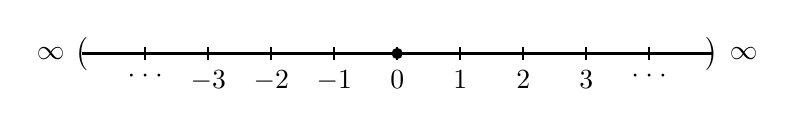
\begin{tikzpicture}[thick,scale=0.8, every node/.style={scale=1}]
        \draw[thick,-] (-5,0) -- (5,0);
        \foreach \x in {-3,-2,-1,0,1,2,3}
            \draw (\x cm,3pt) -- (\x cm,-3pt) node[anchor=north] {$\x$};
        \draw (-4 cm,3pt) -- (-4 cm,-3pt) node[anchor=north] {$\cdot\cdot\cdot$};
        \draw (4 cm,3pt) -- (4 cm,-3pt) node[anchor=north] {$\cdot\cdot\cdot$};
        \filldraw[black] (0,0) circle (2pt);
        \draw node[] at (-5,0) {$\big($};
        \draw node[] at (5,0) {$\big)$};
        \draw node[] at (-5.5,0) {$\infty$};
        \draw node[] at (5.5,0) {$\infty$};
    \end{tikzpicture}
    \caption{Representación del campo real con la recta real.} 
    \label{fig: Campo real}
\end{figure}


\textbf{El campo complejo}

El conjunto de los números complejos se define como
\[
\mathbb{C} \equiv \{a+ib\mid a,b\in\mathbb{R}\}, \quad i \equiv +\sqrt{-i}.
\]
\noindent Para un número complejo $a+ib\in\mathbb{C}$, decimos que $a$ es su \emph{parte real} y que $b$ es su \emph{parte imaginaria}. A los números complejos con parte real nula, i.e., aquellos de la forma $0+ib, b\in\mathbb{R}$, se les conoce como números \emph{imaginarios} . El \emph{complejo conjugado} de un número complejo $a+ib\in\mathbb{C}$ se define como $$\overline{a+ib} = a-ib.$$ Apoyándonos en las operaciones del campo real, podemos definir la suma y multiplicación entre números complejos como\footnote{Nótese que la definición de multiplicación es igual al desarrollo de $(a+ib)(c+id)$ como producto de binomios.}.
\begin{align*}
    (a+ib)+(q+ir) &\equiv(a+q) + i(b+r), \\
    (a+ib)(q+ir)  &\equiv (aq-br) + i(ar+bq).
\end{align*}
 Así mismo, apoyándonos en el campo real, podemos comprobar que estas dos operaciones junto con el conjunto $\mathbb{C}$ forman un campo.  \\

\begin{ejer}\label{ejercicio-3}
    
    Prueba que $\mathbb{C}$, con las operaciones de suma y multiplicación definidas anteriormente, forma un campo.
\end{ejer}

% Geometría del campo complejo. Incluir en la descripción de la figura la nota al pie sobre los números \emph{laterales}\footnote{El mismísimo Gauss hubiera preferido este segundo nombre, ya que creía que era mucho más intuitivo, y que llamarlos \emph{imaginarios} les dotaba de una opacidad misteriosa e innecesaria. Sugiero ver este video introductorio (o la serie completa, llamada Imaginary Numbers Are Real) para perderles el miedo: \url{https://www.youtube.com/watch?v=T647CGsuOVU}.}

Observemos que prácticamente todas las operaciones que realizamos en nuestra vida cotidiana como calcular fechas, dar o recibir cambio, aproximar áreas, repartir comida, etc., toman lugar en un campo. Es decir, las ideas intuitivas que nos formamos durante la educación básica de que la suma siempre debe ser conmutativa y asociativa \textemdash al igual que la multiplicación\textemdash\hspace{0.5mm}, que existe la resta y la división, que el $0$ y el $1$ son números \emph{especiales} en cierto sentido y que siempre se cumple la propiedad de distributividad, son un \emph{hecho} para cualquier estructura de campo. Sin embargo, estas mismas ideas intuitivas \emph{no siempre se cumplen en otros tipos de estructuras algebráicas}\textemdash algunas de las cuales veremos más adelante\textemdash\hspace{0.5mm}, ¡así que no te confíes!

\newpage
\subsection*{Espacios vectoriales} \label{Ssec: Espacios vectoriales}

Un espacio vectorial es una estructura algebráica abstracta que cumple una serie de propiedades específicas que veremos en el siguiente apartado. Dicha estructura tiene una gran variedad de aplicaciones en muchas áreas de las matemáticas, la física, la computación y la biomedicina, por lo cual, para arrancar el curso, es vital su comprensión desde un punto de vista teórico.

\subsubsection*{Definición de espacio vectorial} \label{Def:Espacio_vectorial}

\begin{tcolorbox} \label{Def:Espacio_vectorial}
\underline{Def.} Un \textit{espacio vectorial} sobre un campo\footnote{Ver sec. \ref{Def:Campo}.} $K$ es un conjunto $V$ con dos operaciones (llamadas \textit{adición} o \textit{suma vectorial} y \textit{producto de un vector por un escalar}) que satisfacen las siguientes propiedades:

\begin{center}
\begin{tabular}{lr}
    $\forall\hspace{1.5mm} \mathbf{u},\mathbf{v}\in V \hspace{3mm}\exists \hspace{1.5mm} \mathbf{u}+\mathbf{v}\in V$ & Cerradura de la adición \\ \\ \multirow{2}{0.4\textwidth}{$\forall\hspace{1.5mm} \mathbf{v}\in V, a\in K \hspace{3mm}\exists \hspace{1.5mm} a\mathbf{v}\in V$} & \multirow{2}{0.28\textwidth}{Cerradura del producto de un vector por un escalar} \\ \\ \\
    $\forall\hspace{1.5mm} \mathbf{u},\mathbf{v},\mathbf{w}\in V\hspace{3mm}\mathbf{u}+(\mathbf{v}+\mathbf{w})=(\mathbf{u}+\mathbf{v})+\mathbf{w}$  & Asociatividad de la adición\\ \\
    $\forall\hspace{1.5mm} \mathbf{u},\mathbf{v}\in V\hspace{3mm}\mathbf{u}+\mathbf{v}=\mathbf{v}+\mathbf{u}$ & Conmutatividad de la adición \\ \\
    $\exists \hspace{1.5mm} \mathbf{0}\in V$ t.q. $\mathbf{v}+\mathbf{0}=\mathbf{v}\hspace{3mm}\forall\hspace{1.5mm} \mathbf{v} \in V$ & Elemento identidad de la adición (neutro aditivo) \\ \\
    $\forall\hspace{1.5mm}\mathbf{v}\in V \hspace{3mm}\exists\hspace{1.5mm} -\mathbf{v}\in V$ t.q. $\mathbf{v}+(-\mathbf{v})=\mathbf{0}$ & Elemento inverso de la adición (inverso aditivo) \\ \\
    \multirow{2}{0.35\textwidth}{$a(b\mathbf{v})=(ab)\mathbf{v}\hspace{3mm}\forall a,b\in K, \mathbf{v}\in V$} & \multirow{2}{0.47\textwidth}{Compatibilidad del producto de un vector por un escalar con el producto entre escalares} \\ \\ \\
    \multirow{2}{0.4\textwidth}{$\exists\hspace{1.5mm}1\in K$ \hspace{1.5mm} t.q. $\hspace{1.5mm}1\mathbf{v}=\mathbf{v}\hspace{3mm}\forall\hspace{1.5mm} \mathbf{v}\in V$} & \multirow{2}{0.35\textwidth}{Elemento identidad del producto de un vector por un escalar} \\ \\ \\
    \multirow{2}{0.4\textwidth}{$a(\mathbf{v}+\mathbf{w})=a\mathbf{v}+a\mathbf{w}\hspace{3mm}\forall\hspace{1.5mm} \mathbf{v},\mathbf{w}\in V, a\in K$} & \multirow{2}{0.47\textwidth}{Distributividad del producto de un vector por un escalar con respecto a la adición vectorial}  \\ \\ \\
    \multirow{2}{0.4\textwidth}{$(a+b)\mathbf{v}=a\mathbf{v}+b\mathbf{v}\hspace{3mm}\forall\hspace{1.5mm} a,b\in K, \mathbf{v}\in V$} & \multirow{2}{0.47\textwidth}{Distributividad del producto de un vector por un escalar con respecto a la suma escalar.} \\ \\
\end{tabular}
\end{center}

\hspace{2.5mm} A los elementos $a,b \in K$ del campo utilizado para definir el espacio vectorial se les llama \textit{escalares} y los elementos $\mathbf{u},\mathbf{v},\mathbf{w}\in V$ que cumplen todas las propiedades anteriores son llamados \textit{vectores}. A las propiedades anteriores también se les conoce como \textit{axiomas de espacio vectorial}.

\end{tcolorbox}

Partiendo de esta definición, podemos hacer varias observaciones:

\begin{itemize}
    \item La definición matemática de \textit{vectores} como \textit{elementos cualesquiera de un conjunto V que \textemdash junto con un campo $K$ y las operaciones $+:V\times V\to V$ (suma vectorial) y $\hspace{1mm} \cdot:K\times V\to V$ (producto de un vector por un escalar) \textemdash\hspace{0.5mm} cumplen las propiedades de un espacio vectorial} es muy distinta a la definición de vector como \textit{elemento con magnitud, dirección y sentido (y, más precisamente, que además es invariante bajo rotaciones propias e impropias)} utilizada en algunas áreas de la física, siendo la primera definición más general.
    \item La definición de \textit{espacio vectorial} incluye dos operaciones \textit{nuevas} (con respecto a las operaciones de campo) con una importante diferencia entre ellas: una es sólamente entre los elementos del conjunto $V$ (adición o suma vectorial) y, la otra, entre los elementos del conjunto $V$ y el campo $K$ (producto de un vector por un escalar)\footnote{Más adelante veremos otras operaciones que se pueden definir entre vectores y escalares, pero las dos que hemos visto hasta ahora son las únicas necesarias para \textit{definir} los espacios vectoriales. Por ende, más adelante podremos referirnos a ellas como las operaciones \emph{esenciales} de los espacios vectoriales.}. Sin embargo, \emph{ambas dan como resultado un vector en $V$}.
    \item Así como la definición de \textit{campo} incluye un conjunto $K$ con dos operaciones (suma y producto) entre sus elementos que cumplen propiedades específicas, la definición de \textit{espacio vectorial} incluye un conjunto $V$ y un campo $K$ con dos operaciones (suma vectorial y producto de un vector por un escalar) entre sus elementos que cumplen propiedades específicas. Por simplicidad, al campo se le denota como $K$ y al espacio vectorial, como $V$.
    
\end{itemize}{}

Para complementar la discusión al respecto de qué es un vector y apreciar cómo funcionan las operaciones de los espacios vectoriales (suma vectorial y producto de un vector por un escalar) de manera visual, sugiero ver el siguiente video: \url{https://www.youtube.com/watch?v=fNk_zzaMoSs}.

\subsubsection*{Ejemplos de espacios vectoriales} \label{Ejem:Espacios_vectoriales}

El producto cartesiano del conjunto de los números reales consigo mismo $\mathbb{R}\times\mathbb{R}$ (o $\mathbb{R}^2$) sobre el campo $\mathbb{R}$ es un espacio vectorial, ya que los elementos de $\mathbb{R}^2$ (conocidos como \textit{pares ordenados} o \textit{2-tuplas}) junto con los de $\mathbb{R}$ satisfacen la definición de la sección \ref{Def:Espacio_vectorial}. Usualmente, en geometría analítica, estos pares ordenados se escriben en forma de \emph{coordenadas} $(x,y)$ con $x,y \in \mathbb{R}$ y tienen una correspondencia uno a uno con \emph{puntos} en el plano cartesiano; sin embargo, en álgebra lineal, cuando hablemos de pares ordenados como \emph{vectores} de $\mathbb{R}^2$, es preferible emplear la notación\footnote{A esto se le conoce como \emph{escribir un vector como una columna de matriz} y facilita la notación al momento de hacer productos de matrices por la izquierda con vectores, como haremos más adelante en el curso.} $\textbf{x}=\begin{pmatrix}x_1\\x_2\end{pmatrix}\in\mathbb{R}^2,\hspace{1.5mm}x_1,x_2\in\mathbb{R}$ (lo cual también puede escribirse como $\begin{pmatrix}x_1&x_2\end{pmatrix}^T$ ó, simplemente, $\begin{pmatrix}x_1&x_2\end{pmatrix}$). Estos vectores se pueden representar visualmente mediante una correspondencia uno a uno con \emph{flechas} en el plano cartesiano, las cuales \emph{tienen su cola en el origen} y \emph{su punta en el punto correspondiente a las coordenadas} $(x_1,x_2)$. La suma vectorial se define naturalmente como $\begin{pmatrix}x_1\\x_2\end{pmatrix}+\begin{pmatrix}y_1\\y_2\end{pmatrix}=\begin{pmatrix}x_1+y_1\\x_2+y_2\end{pmatrix}$. El elemento identidad de la suma (neutro aditivo) es el \emph{vector origen} $\mathbf{0}=\begin{pmatrix}0\\0\end{pmatrix}$ y el inverso aditivo de un vector $\mathbf{u}=\begin{pmatrix}u_1\\u_2\end{pmatrix}$ es $\begin{pmatrix}-u_1\\-u_2\end{pmatrix}$, denotado como $-\mathbf{u}$. En este caso, el producto de un vector $\textbf{v}=\begin{pmatrix}v_1\\v_2\end{pmatrix}\in\mathbb{R}^2$ por un escalar $a\in\mathbb{R}$ se define como $a\textbf{v}=a\begin{pmatrix}v_1\\v_2\end{pmatrix} \equiv \begin{pmatrix}av_1\\av_2\end{pmatrix}$ (ó $a\begin{pmatrix}v_1&v_2\end{pmatrix} \equiv \begin{pmatrix}av_1&av_2\end{pmatrix}$) y el elemento de identidad de esta operación es el escalar $1\in\mathbb{R}$.

\vspace{3mm}

El espacio vectorial de $\mathbb{R}^3$ sobre $\mathbb{R}$ se define de manera análoga. Los vectores de $\mathbb{R}^3$ también se pueden representar como flechas que parten del origen de un espacio tridimensional, en una correspondencia uno a uno con las coordenadas del espacio tridimensional. Este tipo de espacios vectoriales se pueden generalizar de manera abstracta (i.e., no visual), como veremos en el siguiente ejemplo.

\vspace{3mm}

El conjunto obtenido al realizar un producto cartesiano de un número entero positivo $n$ de conjuntos $\mathbb{R}$ ($\mathbb{R}\times\mathbb{R}\times...\times\mathbb{R}) = \mathbb{R}^n$ sobre el campo $\mathbb{R}$ también es un espacio vectorial. Sus elementos vectoriales son de la forma $\mathbf{v} = \begin{pmatrix}v_1&v_2& ... & v_n\end{pmatrix}, \hspace{1.5mm} v_i \in \mathbb{R}, \hspace{1.5mm} i \in \{1,2,...,n\}$ y son conocidos como \textit{n-tuplas}\footnote{Nótese que inclusive en el caso $n=1$ el conjunto $\mathbb{R}$ sobre sí mismo forma un espacio vectorial. Es decir, en este caso, $\mathbb{R}$ funciona como conjunto vectorial y como campo.}. Las operaciones entre los vectores de $\mathbb{R}^n$ y con los escalares en $\mathbb{R}$ se definen de manera análoga al ejemplo de $\mathbb{R}^2$. A este tipo de espacios vectoriales les llamamos \textit{espacios vectoriales reales}, de acuerdo con la definición siguiente:

\vspace{1.5mm} 

\begin{tcolorbox}
\underline{Def.} Un \textit{espacio vectorial real} es aquel definido sobre el campo $\mathbb{R}$ (campo real) o, equivalentemente, aquel donde los escalares son números reales.
\end{tcolorbox}{}

El conjunto de todas las funciones polinomiales de una variable real de grado $n$ (i.e., con regla de correspondencia de la forma $f(x) = c_1 x^1 + c_2 x^2 + ... + c_n x^n, \hspace{1.5mm} c_i \in \mathbb{R}, \hspace{1.5mm} i \in \{1,2,...,n\}$) y con un mismo dominio $\mathcal{D}$ forma un espacio vectorial sobre el campo $\mathbb{R}$. Aquí, las definiciones de suma vectorial y de producto de un vector por un escalar se siguen naturalmente de la definición de la suma de funciones $(f+g)(x)\equiv f(x)+g(x)$ y del producto de una función arbitraria $f(x)$ por una función constante $a$, respectivamente, vistas en cálculo \textemdash las cuales aplican para la intersecciones de los dominios. El elemento identidad de la suma vectorial (neutro aditivo) es la función constante cero $f(x)=0\hspace{2.5mm} \forall\hspace{0.5mm}x\in\mathcal{D}$ y el inverso aditivo de una función $g(x)$ es $-g(x)$. Observemos que, en este caso, los \textit{vectores} de nuestro espacio vectorial \textit{son funciones} (en particular, en este ejemplo, son funciones polinomiales).

\vspace{3mm}

El conjunto de todas las funciones de una variable real derivables y con derivada continua (i.e., funciones de clase $C^1$) sobre el campo $\mathbb{R}$ forma un espacio vectorial\footnote{En general, el conjunto de funciones de clase $C^n$ sobre el campo $\mathbb{R}$ forma un espacio vectorial.}. Esto probablemente lo viste de manera implícita en tu curso de cálculo diferencial de una variable, cuando viste los teoremas de derivada de una suma/multiplicación/división de funciones (también conocido como \emph{álgebra de derivadas}) para funciones de este tipo. Las operaciones en este espacio vectorial, así como los elementos identidad (neutros) e inversos, se definen de la misma forma que en el ejemplo de las funciones polinomiales.

\vspace{3mm}

El conjunto $\mathbb{C}\times\mathbb{C}$ ($\mathbb{C}^2$) sobre el campo $\mathbb{C}$ también es un espacio vectorial. Sus vectores son de la forma $\begin{pmatrix}a+ib&c+id\end{pmatrix}$ con $a,b,c,d\in\mathbb{R}$ e $i\equiv+\sqrt{-1}$ (ya que esto implica que $a+ib, c+id\in\mathbb{C}$, es decir, que sus entradas son complejas). El elemento identidad de la suma vectorial es $\mathbf{0}=\begin{pmatrix}0+i0&0+i0\end{pmatrix}$ y el del producto de un vector por un escalar es $1 + i0\in\mathbb{C}$; las operaciones en $\mathbb{C}^2$ y $\mathbb{C}$ se definen como las del ejemplo de $\mathbb{R}^2$ y $\mathbb{R}$. Análogamente, el conjunto $\mathbb{C}^n$ sobre el campo $\mathbb{C}$ es un espacio vectorial: sus vectores tienen $n$ entradas complejas y sus escalares también son complejos. A este tipo de espacio vectorial le llamamos \textit{espacio vectorial complejo}, de acuerdo a la siguiente definición:

\vspace{1.5mm} 
\begin{tcolorbox}
\underline{Def.} Un \textit{espacio vectorial complejo} es aquel definido sobre el campo $\mathbb{C}$ (campo complejo) o, equivalentemente, aquel donde los escalares son números complejos.
\end{tcolorbox}{}

Nota: no podemos visualizar los vectores de $\mathbb{R}^n$ con $n>3$, los de $\mathbb{C}^m$ con $m>1$, ni los del conjunto de funciones de clase $C^1$, etc., como \emph{flechas que parten de un mismo origen}\footnote{Es posible visualizar vectores más abstractos de otras formas: \url{https://www.youtube.com/watch?v=zwAD6dRSVyI}.}. Sin embargo, sí podemos hacer operaciones entre estos vectores de manera análoga a como lo haríamos con vectores de $\mathbb{R}^2$ o $\mathbb{R}^3$, por lo cual trabajar en estos espacios \emph{visualizables} puede ayudarnos a generar intuición sobre espacios vectoriales más abstractos.

\vspace{3mm}
Para ver más ejemplos de espacios vectoriales pueden revisar, por ejemplo, \textit{Linear Algebra} de Friedberg (págs. 8-11.) o \textit{Linear Algebra: A Modern Introduction} de Poole (págs. 430-432), entre otros.

\subsubsection*{Algunos teoremas de espacios vectoriales} \label{Teo:Espacios_vectoriales} 

\begin{teo}\label{teo-1.2}
Sean $\mathbf{x},\mathbf{y},\mathbf{z}$ vectores de $V$ tales que $\mathbf{x}+\mathbf{z}=\mathbf{y}+\mathbf{z}$, entonces $\mathbf{x}=\mathbf{y}$.

\begin{proof}
Ya que $\mathbf{z}$ es un vector de $V\implies$ $\exists\hspace{2mm} \mathbf{-z}\in V$ tal que $\mathbf{z} + (-\mathbf{z}) = \mathbf{0}$, por la propiedad de existencia de inversos aditivos de los espacios vectoriales. Sumando este elemento $-\mathbf{z}$ a cada lado de la igualdad inicial, tenemos que $$\mathbf{x}+\mathbf{z}=\mathbf{y}+\mathbf{z}\iff\mathbf{x}+\mathbf{z}+ (-\mathbf{z})=\mathbf{y}+\mathbf{z}+ (-\mathbf{z})\iff\mathbf{x}+(\mathbf{z}+ (-\mathbf{z}))=\mathbf{y}+(\mathbf{z}+ (-\mathbf{z}))\iff$$ $$ \mathbf{x}+\mathbf{0}=\mathbf{y}+\mathbf{0}\iff\mathbf{x}=\mathbf{y},$$

\noindent donde en la tercera igualdad se aplicó la propiedad asociativa de la suma vectorial, en la cuarta igualdad se aplicó la propiedad de existencia de los inversos aditivos y, en la última, se aplicó la propiedad de existencia de neutro aditivo.
\end{proof}
\end{teo}

\noindent Al teorema anterior se le conoce como \emph{Ley de cancelación para la suma vectorial} y con él se puede demostrar la unicidad del nuetro aditivo y de los inversos aditivos.

\begin{teo}\label{teo-1.3}
Sea $V$ sobre $K$ un espacio vectorial arbitrario con $\mathbf{v}\in V$ y $a\in K$, entonces se verifica que:

\begin{enumerate}
    \item $0\mathbf{v}=\mathbf{0}$
    \item $a\mathbf{0}=\mathbf{0}$
    \item $(-a)\mathbf{v}=-(a\mathbf{v})=a(-\mathbf{v})$
\end{enumerate}

\begin{proof}
\begin{enumerate}
    \item $0\mathbf{v}+0\mathbf{v}=(0+0)\mathbf{v}=0\mathbf{v}=0\mathbf{v}+\mathbf{0}\iff0\mathbf{v}=\mathbf{0}$, donde se aplicaron las propiedades de distributividad del producto de un vector por un escalar con respecto a la suma \emph{escalar}, existencia del neutro aditivo y la ley de cancelación de la suma vectorial (Teorema \ref{teo-1.2}).
    \item $a\mathbf{0}+a\mathbf{0}=a(\mathbf{0}+\mathbf{0})=a\mathbf{0}=a\mathbf{0}+\mathbf{0}\iff a\mathbf{0}=\mathbf{0}$, donde se aplicaron las propiedades de distributividad del producto de un vector por un escalar con respecto a la adición \emph{vectorial}, existencia del neutro aditivo y la ley de cancelación de la suma vectorial.
    \item Por el primer inciso y por distributividad, $\mathbf{0} = (0)\mathbf{v} = (a+(-a))\mathbf{v}=a\mathbf{v}+(-a)\mathbf{v}$\footnote{La existencia de $-a\in K$ está asegurada ya que $K$ es un campo (ver sec. \ref{Def:Campo}).}, por lo cual $a\mathbf{v}+(-a)\mathbf{v}=\mathbf{0}$. Por otro lado, por la propiedad de cerradura del producto de un vector por un escalar $a\mathbf{v}\in V$ y, por la existencia de inversos aditivos, $\exists\hspace{1mm}-(a\mathbf{v})\in V$ tal que $a\mathbf{v}+[-(a\mathbf{v})]=\mathbf{0}$. Por lo tanto, tenemos que $\mathbf{0}=\mathbf{0}\iff a\mathbf{v}+(-a)\mathbf{v}=a\mathbf{v}+[-(a\mathbf{v})]\iff (-a)\mathbf{v}=-(a\mathbf{v})$ por la ley de cancelación. En particular, $(-1)\mathbf{v}=-\mathbf{v}$; por la propiedad de compatibilidad del producto de un vector por un escalar con el producto entre escalares, se sigue que $a(-\mathbf{v})=a[(-1)\mathbf{v}]=[a(-1)]\mathbf{v}=(-a)\mathbf{v}=-(a\mathbf{v})$.
\end{enumerate}
\end{proof}
\end{teo}

\newpage
\subsubsection*{Interpretación geométrica de las operaciones esenciales de los espacios vectoriales} \label{Sssec:Interpretación geométrica de las operaciones de los espacios vectoriales}

Como se mencionó en una nota al final de la sección \ref{Ejem:Espacios_vectoriales} \hspace{1.5mm}\textemdash de la cual retomaremos muchas ideas a continuación\textemdash, podemos desarrollar nuestra intuición sobre muchos temas del álgebra lineal trabajando en espacios vectoriales \emph{visualizables}, para luego extenderla a espacios vectoriales más generales. Por ende, ahora haremos hincapié en la interpretacción geométrica de las operaciones de suma vectorial y producto de un vector por un escalar en los espacios vectoriales reales $\mathbb{R}^2$ y $\mathbb{R}^3$, así como en el espacio vectorial complejo $\mathbb{C}$. Antes de empezar, necesitamos recordar la siguiente definición.

\vspace{1.5mm}

\begin{tcolorbox}
 \underline{Def.} Un \emph{par ordenado} (o \emph{$2$-tupla}) es un par de números $(a,b)$ en donde el orden de los números importa; mátematicamente, decimos que el par ordenado $(a,b)\neq (b,a)\iff b\neq a$\footnote{Observemos que esto implicaría que $(a,b)=(b,a)\iff b=a$, lo cual tiene sentido ya que, si ambos números son el mismo, es imposible distinguir el orden. Esta es una definición equivalente de par ordenado.}.
\end{tcolorbox}{}

\subsubsection*{En el espacio vectorial real \texorpdfstring{$\mathbb{R}^2$}{TEXT}} \label{Ejem:En_R^2}

En geometría analítica aprendimos que, con la ayuda de un sistema de coordenadas, podemos formar una correspondencia uno a uno (o \emph{biunívoca}) entre los pares ordenados $(a,b)$ de entradas reales\footnote{Es decir, con $a,b\in\mathbb{R}$.} y los puntos del plano cartesiano $\mathbb{R}\times\mathbb{R}$. En particular, si tomamos el sistema de coordenadas cartesianas, entonces a cualquier par ordenado de entradas reales $(a,b)$ le corresponde un punto en el plano cartesiano $\mathbb{R}\times\mathbb{R}$ con coordenadas cartesianas $(a,b)$, y vice versa. De manera análoga, en álgebra lineal, cada vector $\begin{pmatrix}a&b\end{pmatrix} \in \mathbb{R}^2$ tiene una correspondencia biunívoca con una flecha en el plano cartesiano que tiene cola en el origen y punta en la coordenada cartesiana $(a,b)$ correspondiente. Ambas correspondencias se muestran en la Figura \ref{fig:Correspondencias_del_plano_cartesiano}.

\begin{figure}[h!]
    \centering
    \begin{tikzpicture}[thick,scale=0.8, every node/.style={scale=1}]
        \draw[thick,<->] (-4,0) -- (4,0);
        \draw[thick,<->] (0,-4) -- (0,4);
        \draw[step=1cm,gray,very thin,dashed] (-3.9,-3.9) grid (3.9,3.9);
        \foreach \x in {1,2,3}
            \draw (\x cm,1pt) -- (\x cm,-1pt) node[anchor=north] {$\x$};
        \foreach \y in {1,2,3}
            \draw (1pt,\y cm) -- (-1pt,\y cm) node[anchor=east] {$\y$};
        \foreach \x in {-3,-2,-1}
            \draw (\x cm, 1pt) -- (\x cm, -1pt);
        \foreach \y in {-3,-2,-1}
            \draw (1pt,\y cm) -- (-1pt,\y cm);
        \filldraw[black] (0,0) circle (2pt) node[] at (-0.6,0.35) {\small{$(0,0)$}};
        \filldraw[NARANJA] (2,3) circle (2pt) node[anchor=south east] {$(2,3)$};
        \draw[ROJO,very thick,->] (0,0) -- (2,3) node[] at (3,2.5) {$\begin{pmatrix} 2 & 3 \end{pmatrix}$};
        \filldraw[VERDE] (-3.5,-2) circle (2pt) node[anchor=south east]{$(-3.5,-2)$};
        \draw[AZUL,very thick,->] (0,0) -- (-3.5,-2) node[] at (-2,-2.5) {$\begin{pmatrix} -3.5 & -2 \end{pmatrix}$};
    \end{tikzpicture}
    \caption{Ejemplo de representación de pares ordenados y vectores en el plano cartesiano. Los pares ordenados $(-3.5,-2)$ y $(2,3)$ se representan mediante puntos que corresponden precisamente a las coordenadas cartesianas $(-3.5,-2)$ y $(2,3)$, respectivamente, mientras que los vectores $\protect\begin{pmatrix} -3.5 & -2 \protect\end{pmatrix}$ y $\protect\begin{pmatrix} 2 & 3 \protect\end{pmatrix}$ son representados por flechas que tienen su cola en el origen del plano cartesiano y su punta en las coordenadas $(-3.5,-2)$ y $(2,3)$, respectivamente.} 
    \label{fig:Correspondencias_del_plano_cartesiano}
\end{figure}

\vspace{3mm}
\textbf{Suma vectorial}
\vspace{3mm}

    En este espacio, la suma vectorial se define como $\begin{pmatrix}a&b\end{pmatrix}+\begin{pmatrix}c&d\end{pmatrix}\equiv\begin{pmatrix}a+c&b+d\end{pmatrix}$. Podemos calcular, por ejemplo, la suma $\begin{pmatrix}2&1\end{pmatrix}+\begin{pmatrix}1&3\end{pmatrix}=\begin{pmatrix}3&4\end{pmatrix}$. Los tres vectores mencionados se muestran en la Figura \ref{fig:Suma_vectorial}.

\begin{figure}[h!]
    \centering
    \begin{tikzpicture}[thick,scale=1.6, every node/.style={scale=1}]
        \draw[thick,->] (0,0) -- (4.5,0);
        \draw[thick,->] (0,0) -- (0,4.5);
        \draw[step=1cm,gray,thin,dashed] (0,0) grid (4.4,4.4);
        \foreach \x in {0,1,2,3,4}
            \draw (\x cm,1pt) -- (\x cm, -1pt) node[anchor=north] {$\x$};
        \foreach \y in {1,2,3,4}
            \draw (1pt,\y cm) -- (-1pt,\y cm) node[anchor=east] {$\y$};
        
            \draw[ROJO,very thick,->] (0,0) -- (2,1) node[] at (2.05,0.5){$\begin{pmatrix} 2 & 1 \end{pmatrix}$};
            \draw[AZUL,very thick,->] (0,0) -- (1,3) node[] at (0.55,3) {$\begin{pmatrix} 1 & 3 \end{pmatrix}$};
            \draw[violet,very thick,->] (0,0) -- (3,4) node[] at (3,4.2) {$\begin{pmatrix} 3 & 4 \end{pmatrix}$};
            \draw[] node[] at (4.2,4.2) {\textbf{a)}};
            \draw[black,thick,->]  (5,2) -- (5.5,2);
    \end{tikzpicture} \hspace{0.5cm} \begin{tikzpicture}[thick,scale=1.6, every node/.style={scale=1}]
        \draw[thick,->] (0,0) -- (4.5,0);
        \draw[thick,->] (0,0) -- (0,4.5);
        \draw[step=1cm,gray,thin,dashed] (0,0) grid (4.4,4.4);
        \foreach \x in {0,1,2,3,4}
            \draw (\x cm,1pt) -- (\x cm, -1pt) node[anchor=north] {$\x$};
        \foreach \y in {1,2,3,4}
            \draw (1pt,\y cm) -- (-1pt,\y cm) node[anchor=east] {$\y$};
            \draw[ROJO,very thick,->] (0,0) -- (2,1) node[] at (2.05,0.5){$\begin{pmatrix} 2 & 1 \end{pmatrix}$};
            \draw[AZUL,dashed,->] (2,1) -- (3,4) node[] at (3,2.4) {$\begin{pmatrix} 1 & 3 \end{pmatrix}$};
            \draw[AZUL,very thick,->] (0,0) -- (1,3) node[] at (0.55,3) {$\begin{pmatrix} 1 & 3 \end{pmatrix}$};
            \draw[ROJO,dashed,->] (1,3) -- (3,4) node[] at (1.7,3.8) {$\begin{pmatrix} 2 & 1 \end{pmatrix}$};
            \draw[violet,very thick,->] (0,0) -- (3,4) node[] at (3,4.2) {$\begin{pmatrix} 3 & 4 \end{pmatrix}$};
            \draw[] node[] at (4.2,4.2) {\textbf{b)}};
    \end{tikzpicture}
        \caption{Interpretación geométrica de la suma vectorial en el espacio vectorial real $\protect\mathbb{R}^2$. En la subfigura $\textbf{a)}$ se observan los vectores $\protect\begin{pmatrix} 1 & 3 \protect\end{pmatrix}$ y $\protect\begin{pmatrix} 2 & 1 \protect\end{pmatrix}$, así como el vector resultante de la suma de los dos anteriores, $\protect\begin{pmatrix} 3 & 4 \protect\end{pmatrix}$. En la subfigura $\textbf{b)}$ observamos la llamada \emph{Ley del paralelogramo} para la suma de dos vectores.}
    \label{fig:Suma_vectorial}
\end{figure}

    Observemos que, visualmente, esto corresponde a trazar uno de los vectores en el plano cartesiano y luego trazar el otro colocando la cola en la punta del vector anterior, como si ése fuese su origen. Nótese que no importa cuál vector trazamos primero y cuál después, lo cual concuerda con la conmutatividad de la suma vectorial (esta misma interpretación geométrica es válida para la suma de tres o más vectores de $\mathbb{R}^2$: basta irlos sumando de dos en dos vectores); a esto se le conoce como la \textit{Ley del paralelogramo}. En particular, $\forall\hspace{0.5mm} \mathbf{v} \in \mathbb{R}^2$, $\mathbf{0}+\mathbf{v}=\mathbf{v}$, lo cual concuerda con el hecho de que el vector $\mathbf{v}$ corresponda a una flecha con cola en el origen.

\vspace{3mm}
\textbf{Producto de un vector por un escalar}
\vspace{3mm}

        En este espacio, el producto de un vector por un escalar se define como $c\begin{pmatrix}a&b\end{pmatrix}\equiv\begin{pmatrix}ca&cb\end{pmatrix}$. Podemos calcular, por ejemplo, los productos $(\frac{1}{2})\begin{pmatrix}2&2\end{pmatrix}=\begin{pmatrix}1&1\end{pmatrix}$ y $(-1.2)\begin{pmatrix}1&3\end{pmatrix}=\begin{pmatrix}-1.2&-3.6\end{pmatrix}$. La representación gráfica de estas operaciones se muestra en la Figura \ref{fig:Producto_de_un_vector_por_un_escalar}.

\begin{figure}[h!]
    \centering
    \begin{tikzpicture}[thick,scale=0.8, every node/.style={scale=1}]
        \draw[thick,<->] (-4,0) -- (4,0);
        \draw[thick,<->] (0,-4) -- (0,4);
        \draw[step=1cm,gray,thin,dashed] (-3.9,-3.9) grid (3.9,3.9);
        \foreach \x in {1,2,3,4}
            \draw (\x cm,1pt) -- (\x cm, -1pt) node[anchor=north] {$\x$};
        \foreach \y in {1,2,3,4}
            \draw (1pt,\y cm) -- (-1pt,\y cm) node[anchor=east] {$\y$};
            \draw[ROJO,very thick,->] (0,0) -- (2,2) node[anchor=west] {$\begin{pmatrix} 2 & 2 \end{pmatrix}$};
            \draw[AZUL,very thick,->,opacity=0.7] (0,0) -- (1,3) node[anchor=south west] {$\begin{pmatrix} 1 & 3 \end{pmatrix}$};
            \draw[black,thick,->]  (5,0) -- (5.7,0);
            \draw[] node[] at (3.5,3.5) {\textbf{a)}};
            \end{tikzpicture} \hspace{0.5mm} \begin{tikzpicture}[thick,scale=0.8, every node/.style={scale=1}]
        \draw[thick,<->] (-4,0) -- (4,0);
        \draw[thick,<->] (0,-4) -- (0,4);
        \draw[step=1cm,gray,thin,dashed] (-3.9,-3.9) grid (3.9,3.9);
        \foreach \x in {1,2,3,4}
            \draw (\x cm,1pt) -- (\x cm, -1pt) node[anchor=north] {$\x$};
        \foreach \y in {1,2,3,4}
            \draw (1pt,\y cm) -- (-1pt,\y cm) node[anchor=east] {$\y$};
            \draw[ROJO,very thick,opacity=0.7,->] (0,0) -- (1,1) node[] at (2.1,0.65) {$\begin{pmatrix} 1 & 1 \end{pmatrix}$};
            \draw[AZUL,very thick,->] (0,0) -- (-1.2,-3.6) node[] at (-3,-3.4) {$\begin{pmatrix} -1.2 & -3.6 \end{pmatrix}$};
            \draw[ROJO,thin,dashed,->] (0,0) -- (2,2); 
            \draw[AZUL,thin,dashed,->,opacity=0.7] (0,0) -- (1,3); 
            \draw[] node[] at (3.5,3.5) {\textbf{b)}};
    \end{tikzpicture}
    \caption{Interpretación geométrica del producto de un vector por un escalar en el espacio vectorial real $\mathbb{R}^2$. Comparando las subfiguras $\textbf{a)}$ y $\textbf{b)}$ observamos que, en caso de que se multiplique a un vector de $\mathbb{R}^2$ por un escalar de $\mathbb{R}$, es posible que la longtitud del vector cambie y que su sentido se invierta, pero su dirección no cambia.}
    \label{fig:Producto_de_un_vector_por_un_escalar}
\end{figure}


        Como podemos observar, el primer producto redujo la longitud del vector sin cambiar su sentido, mientras que el segundo producto aumentó la longitud del vector, a la vez que invirtió su sentido; sin embargo, en ambos casos, el producto de un vector por un escalar no cambió la \emph{dirección} de los vectores\textemdash es decir, los mantuvo en la misma \emph{línea}. En general, si el escalar $c\in\mathbb{R}$ que multiplica al vector tiene $|c|>1$, lo \emph{alarga}; si tiene $|c|<1$, lo acorta; finalmente, si tiene $|c|=1$, no cambia su longitud. Por este cambio de longitud es que al producto de un vector por un escalar también se le conoce por el nombre \emph{reescalamiento}. Además, si $c>0$, el vector mantiene su misma dirección y sentido (sigue en la misma línea y apunta hacia el mismo lado) mientras que, si $c<0$, el vector conserva su dirección pero se invierte su sentido (sigue en la misma línea pero apunta hacia el lado opuesto); si $c=0$ entonces el vector automáticamente se convierte en el vector nulo $\begin{pmatrix}0&0\end{pmatrix}$, como se demostró algebráicamente en el primer inciso del Teorema \ref{teo-1.2} Para visualizar las operaciones de adición vectorial y producto de un vector por un escalar de forma interactiva, recomiendo la sección \textbf{Vector Algebra and Geometry} de \url{https://textbooks.math.gatech.edu/ila/vectors.html}, así como la ilustración interactiva \url{http://immersivemath.com/ila/ch02_vectors/ch02.html#fig_vec_scaling}.

    Así, en general, si combinamos las operaciones de suma vectorial y producto de un vector por un escalar, visualmente lo que estaremos haciendo será \emph{combinar líneas} con diferentes longitudes, direcciones y sentidos en el plano cartesiano. 

\vspace{3mm}

        Nota: El vector nulo $\mathbf{0}=\begin{pmatrix}0&0\end{pmatrix}$ (también llamado \emph{vector origen}) no tiene longitud, ya que es el único donde la cola y la punta de su flecha coinciden. Además, se dice que tampoco tiene dirección ni sentido\footnote{Alternativamente, se dice que tiene \emph{todas las direcciones} y \emph{todos los sentidos simultáneamente}: en la práctica, ambas interpretaciones son equivalentes, pero la primera puede ser más fácil de asimilar.}. Si asumimos que este vector no tiene longitud, dirección ni sentido, entonces queda claro por qué cualquier reescalamiento de este vector no lo modifica, como se demostró en el segundo inciso del Teorema \ref{teo-1.2}.

\subsubsection*{En el espacio vectorial real \texorpdfstring{$\mathbb{R}^3$}{TEXT}}

La suma vectorial y el producto de un vector por un escalar (o \emph{reescalamiento}) en el espacio vectorial real $\mathbb{R}^3$ tienen la misma interpretación geométrica que en $\mathbb{R}^2$, con una dimensión extra añadida. Esto es de esperarse, ya que las definiciones de estas operaciones y las correspondencias entre vectores y flechas que salen del origen a una coordenada específica son análogas en ambos espacios vectoriales.

\subsubsection*{En el espacio vectorial complejo \texorpdfstring{$\mathbb{C}$}{TEXT}}

Como hemos visto, el plano cartesiano nos sirve para representar vectores con dos entradas reales. De manera similar, el \emph{plano complejo} \textemdash con un eje de números \emph{reales} (por convención, el horizontal) y otro eje perpendicular a él de números \emph{imaginarios}\footnote{Los números imaginarios son aquellos números complejos con la parte real igual a cero, i.e. $0+ib=ib\in\mathbb{C}$, donde $b$ es un número real. En otras palabras, son el resultado de multiplicar el número imaginario $i$ por cualquier número real.}\textemdash\hspace{0.5mm} nos sirve para representar vectores con una entrada compleja. Así, cada vector de una entrada compleja $\begin{pmatrix}a+ib\end{pmatrix}$ con $a,b\in\mathbb{R}$ tiene una correspondencia uno a uno con una flecha con cola en el origen del plano y flecha en la coordenada $(a,ib)$ del plano complejo, la cual corresponde a, desde el origen, moverse $a$ unidades sobre el eje real y $b$ unidades sobre el eje imaginario.

\vspace{3mm}
\textbf{Suma vectorial}
\vspace{3mm}

De la definición de suma vectorial $\begin{pmatrix}a+ib\end{pmatrix}+\begin{pmatrix}c+id\end{pmatrix}\equiv\begin{pmatrix}(a+c)+(b+d)i\end{pmatrix}$ se deduce que la suma vectorial entre vectores de $\mathbb{C}$ tiene la misma interpretación geométrica que aquella entre vectores de $\mathbb{R}^2$. Por ejemplo, si calculamos $\begin{pmatrix}1+2i\end{pmatrix}+\begin{pmatrix}3+2i\end{pmatrix}=\begin{pmatrix}4+4i\end{pmatrix}$, podemos representarlo visulamente en la Figura \ref{fig:Suma_vectorial_compleja}.

\begin{figure}[h!]
    \centering
    \begin{tikzpicture}
        \draw[thick,->] (0,0) -- (5,0);
        \draw[thick,->] (0,0) -- (0,5);
        \draw[step=1cm,gray,thin,dashed] (0,0) grid (4.9,4.9);
        \foreach \x in {1,2,3,4}
            \draw (\x cm,1pt) -- (\x cm, -1pt) node[anchor=north] {$\x$};
        \draw (1pt, 1cm) -- (-1pt, 1 cm) node[anchor=east] {$i$};
        \foreach \y in {2,3,4}
            \draw (1pt,\y cm) -- (-1pt,\y cm) node[anchor=east] {$\y i$};
            \draw[AZUL,very thick,->] (0,0) -- (1,2) node[] at (0.8,2.6) {$\begin{pmatrix} 1 + 2i \end{pmatrix}$};
            \draw[ROJO,thin,dashed,->] (1,2) -- (4,4) node[] at (2.4,3.8) {$\begin{pmatrix} 3 + 2i \end{pmatrix}$};
            \draw[ROJO,very thick,->] (0,0) -- (3,2) node[] at (3.1,1.2) {$\begin{pmatrix} 3 + 2i \end{pmatrix}$};
            \draw[AZUL,thin,dashed,->] (3,2) -- (4,4) node[] at (4.2,2.6) {$\begin{pmatrix} 1 + 2i \end{pmatrix}$};
        \draw[violet,very thick,->] (0,0) -- (4,4) node[anchor=south west] {$\begin{pmatrix} 4 + 4i \end{pmatrix}$};
    \end{tikzpicture}
    \caption{Interpretación geométrica de la suma vectorial en el espacio vectorial complejo $\mathbb{C}$. Observamos que, al igual que en el caso del espacio vectorial real $\mathbb{R}^2$, se cumple la \emph{Ley del paralelogramo}.}
    \label{fig:Suma_vectorial_compleja}
\end{figure}



\vspace{3mm}
\textbf{Producto de un vector por un escalar}
\vspace{3mm}

Por definición, el producto de un vector por un escalar es $(q+ir)\begin{pmatrix}s+it\end{pmatrix}\equiv\begin{pmatrix}(qs-rt)+i(qt+rs)\end{pmatrix}$.

Notemos que, en particular, si la parte imaginaria del escalar es nula (i.e., si $r=0$), entonces el escalar es un número real y el producto resultante es $(q)\begin{pmatrix}s+it\end{pmatrix}\equiv\begin{pmatrix}(qs)+(qt)i\end{pmatrix}$, por lo cual geométricamente sólo se produce un reescalamiento totalmente análogo al discutido en la sección \ref{Ejem:En_R^2}.

En cambio, ahora observemos qué sucede si la parte real del escalar es nula y la parte imaginaria es igual a $1$ (i.e., si multiplicamos por el escalar $i$). Tomemos, por ejemplo, al vector $\begin{pmatrix}2+2i\end{pmatrix}$. Al hacer el producto de este vector por $i$ obtenemos $\begin{pmatrix}-2+2i\end{pmatrix}$. Si, en cambio, hacemos el producto de este mismo vector por el escalar $-i$, obtenemos como resultado $(-i)\begin{pmatrix}2+2i\end{pmatrix}=\begin{pmatrix}2-2i\end{pmatrix}$. Ambas operaciones se muestran de manera visual en la Figura \ref{fig:Producto_de_un_vector_complejo_por_i}.

\begin{figure}[h!]
    \centering
    \begin{tikzpicture}
        \draw[thick,<->] (-3.5,0) -- (3.5,0);
        \draw[thick,<->] (0,-3.5) -- (0,3.5);
        \draw[step=1cm,gray,thin,dashed] (-3.4,-3.4) grid (3.4,3.4);
        \foreach \x in {1,2}
            \draw (\x cm,1pt) -- (\x cm, -1pt) node[anchor=north] {$\x$};
            \draw (1pt,1 cm) -- (-1pt,1 cm) node[anchor=east] {$i$};
            \draw (1pt,2 cm) -- (-1pt,2 cm) node[anchor=east] {$2i$};
            \draw[darkgray,very thick,opacity=0.8,->] (0,0) -- (2,2) node[anchor=south west] {$\begin{pmatrix} 2 & 2i \end{pmatrix}$};
            \draw[gray,very thick,opacity=0.9,->] (0,0) -- (-2,2) node[anchor=south east] {$\begin{pmatrix} -2 & 2i \end{pmatrix}$};
            \draw[darkgray,very thick,->] (0,0) -- (2,-2) node[anchor=north west] {$\begin{pmatrix} 2 & -2i \end{pmatrix}$};
    \end{tikzpicture}
    \caption{Interpretación geométrica del producto de un vector complejo por los números imaginarios $i$ y $-i$. En este caso, nuestro vector base es $\protect\begin{pmatrix} 2 & 2i \protect\end{pmatrix}$. El producto de este vector por el escalar $i$ resulta en el vector $\protect\begin{pmatrix} -2 & 2i \protect\end{pmatrix}$, lo cual puede ser interpretado geométricamente como una rotación discreta de $\frac{\pi}{2}$ radianes. Así observamos que, en cambio, el producto de nuestro vector base $\protect\begin{pmatrix} 2 & 2i \protect\end{pmatrix}$ por $-i$ se puede interpretar geométricamente como una rotación discreta de $-\frac{\pi}{2}$ radianes.}
    \label{fig:Producto_de_un_vector_complejo_por_i}
\end{figure}

   Aquí vemos que hacer el producto de un vector por el escalar $i$ \emph{equivale a hacer una rotación de $90^\circ$ ó $\frac{\pi}{2}$ radianes}. Análogamente, el producto de un vector por el escalar $-i$ equivale a hacer una rotación de $-90^\circ$ ó $-\frac{\pi}{2}$ radianes. Esto tiene sentido ya que $-i=-1(i)=i(-1)$ lo cual implica que, debido a la compatibilidad del producto de un vector por un escalar con el producto entre escalares, es lo mismo multiplicar un vector por $(-i)$ a multiplicarlo por $i$ y después por -1, o vice versa: el razonamiento geométrico correspondiente es que da lo mismo rotar un vector $-\frac{\pi}{2}$ radianes a rotarlo $\frac{\pi}{2}$ radianes y después invertir su sentido, o primero invertir su sentido y después rotarlo $\frac{\pi}{2}$ radianes. 

   ¿Y si multiplicamos un vector de $\mathbb{C}$ por un escalar $ai$ con $a\neq 0,1$? Ya que $ai\begin{pmatrix}b + ic\end{pmatrix}=\begin{pmatrix}-ac+i(ab)\end{pmatrix}=a\begin{pmatrix}-c+ib\end{pmatrix}=a(i\begin{pmatrix}b+ic\end{pmatrix})$ \textemdash es decir, por la compatibilidad entre productos\textemdash\hspace{0.5mm} podemos deducir que hacer el producto de un vector complejo por un número imaginario arbitrario $ai$ tendrá dos consecuencias: rotarlo de acuerdo a $i$ ($\frac{\pi}{2}$ radianes a contrarreloj) y reescalarlo de acuerdo al valor de $a$ (invirtiendo el sentido si $a<0$). En este último caso donde $a$ es negativo, ya que $ai=|a|(-i)=(-i)|a| \hspace{3mm}\forall\hspace{1.5mm} a<0$, también podríamos pensar que se rota al vector complejo de acuerdo a $-i$ ($\frac{\pi}{2}$ radianes en el sentido de las manecillas) y se reescala de acuerdo al valor absoluto de $a$: ambos razonamientos son equivalentes.

Dicho lo anterior, estamos listos para el caso más general: multiplicar un vector complejo $\begin{pmatrix}s+it\end{pmatrix}$ por un escalar complejo $q+ir$ con $q,r\neq0$ \emph{reescalará} el vector en el plano complejo y lo \emph{rotará} en el sentido correspondiente al signo de $r$. Es decir que, en los espacios vectoriales complejos, los escalares no sólamente pueden \emph{reescalar} vectores, sino que también los pueden \emph{rotar}\footnote{El asunto de las \emph{magnitudes específicas} de estos reescalamientos y rotaciones \textemdash el cual se complica para escalares complejos en general\textemdash\hspace{0.5mm} será precisado más adelante.}.

\subsubsection*{Espacios vectoriales} \label{Ejer:Espacios_vectoriales}

\begin{enumerate}
%    \item En la definición de espacio vectorial de la sección \ref{Def:Espacio_vectorial} no se especifica que los resultados de las operaciones $\mathbf{u}+\mathbf{v}$ (en la propiedad de \textit{cerradura de la adición}) ni $a\mathbf{v}$ (en \textit{cerradura del producto de un vector por un escalar}) sean únicos. Tampoco se especifica que el elemento identidad de la adición ($\mathbf{0}$), el elemento identidad del producto de un vector por un escalar ($1$), ni los elementos inversos de la adición de cada vector $\mathbf{v}$ ($-\mathbf{v}$) sean únicos. Demuestra que todos los elementos mencionados anteriormente son únicos. 
    \item Sea $K$ un campo arbitrario. ¿Siempre puede definirse un espacio vectorial de $K$ (como conjunto vectorial) sobre sí mismo (como campo)? Si sí, demuéstralo. Si no, da un contraejemplo (Nota: repasa los axiomas de campo y ten cuidado con tu notación). 
    \item Explica por qué \textbf{no} puede existir un espacio vectorial con vectores reales en $\mathbb{R}^n$ sobre el campo $\mathbb{C}$, pero sí puede haber un espacio vectorial con vectores complejos en $\mathbb{C}^n$ sobre el campo $\mathbb{R}$. 
    \item Sea $K$ un campo arbitrario. Demuestra que $K^n$ sobre $K$ es un espacio vectorial, con $n\in\mathbb{N}$. 
\end{enumerate}

\subsubsection*{Interpretacción geométrica de los espacios vectoriales}

\begin{enumerate}
        \item Define las variables $a,b,c,d,e\in\mathbb{R}$ de acuerdo a los últimos 5 dígitos de tu número de cuenta. Calcula algebráicamente al vector $\begin{pmatrix}a & b\end{pmatrix}+c\begin{pmatrix}d & e\end{pmatrix}$ y muestra gráficamente al vector resultante aplicando la Ley del paralelogramo. 
                \item Como vimos en la sección \ref{Subsec:Interpretación_geométrica_de_las_operaciones_de_los_espacios_vectoriales}, la suma de dos vectores $\mathbf{v},\mathbf{u}\in\mathbb{R}^2$ sobre $\mathbb{R}$ se puede representar geométricamente con ayuda de un paralelogramo en el plano cartesiano, en donde la diagonal del paralelogramo que sale del origen es igual al vector resultante de la suma $\mathbf{u}+\mathbf{v}$ ó $\mathbf{v}+\mathbf{u}$ (ver, e.g., la Figura \ref{fig:Suma_vectorial}). Muestra intuitivamente que si transportamos a la \emph{otra} diagonal del paralelogramo hasta el origen (lo cual se puede hacer de dos maneras distintas), obtenemos la representación del vector resultante de la resta $\mathbf{u}-\mathbf{v}$ ó $\mathbf{v}-\mathbf{u}$. 
                        \item Muestra intuitivamente que el punto de intersección de las diagonales del paralelogramo mencionado en el ejercicio anterior es igual a la punta del vector $\frac{1}{2}(\vec{u}+\vec{v})$. 
                                \item Elige los dos últimos dígitos de tu número de cuenta y llámalos $q$ y $r$, respectivamente. Al segundo y tercer dígito de tu número de cuenta, llámalos $s$ y $t$. Dibuja el vector complejo $\begin{pmatrix} q + ir \end{pmatrix}\in\mathbb{C}$ en el plano complejo. Explica qué le pasaría a este vector si realizáramos su producto por los escalares complejos $s+it$, $-s+it$, $s-it$ y $-s-it$. 
\end{enumerate}

\subsubsection*{Subespacios vectoriales}

\begin{enumerate}
    \item En la página 17 del libro \textit{Linear Algebra} de Friedberg, la definición de un subespacio vectorial incluye una cuarta propiedad que deben cumplir (la de existencia de inversos aditivos), la cual no incluí en las notas del curso, ya que es redundante. Explica por qué se puede desechar esta cuarta propiedad sin afectar la definición de subespacio vectorial. 
    \item Demuestra que el conjunto $\{\begin{pmatrix} a&2a&3a \end{pmatrix}\in\mathbb{R}^3\mathop|\mathop a\in\mathbb{R}\}$ sobre el campo $\mathbb{R}$ es un subespacio vectorial de $\mathbb{R}^3$. ¿Qué representa este conjunto visualmente en $\mathbb{R}^3$? 
    \item Demuestra que el espacio vectorial de todas las funciones polinomiales de una variable real de grado $n$ es un subespacio vectorial del espacio vectorial de todas las funciones reales de una variable de clase $C^m$ para toda $n \geq m$. 
    \item Demuestra que el espacio vectorial de todas las funciones de una variable real que son derivables y tienen derivada continua (de clase $C^1$) sobre $\mathbb{R}$ es un subespacio vectorial del espacio vectorial de todas las funciones reales continuas (de clase $C^0$) de una variable sobre $\mathbb{R}$. ¿Cómo generalizarías este resultado a que las de clase $C^i$ formen un subespacio de las de clase $C^n$ con $i>n$ sobre el mismo campo $\mathbb{R}$? Argumenta. 
    \item Demuestra el Teorema \ref{teo-2.2} (ver sec. \ref{Teo:Subespacios_vectoriales}). 
\end{enumerate}

\end{document}
